\documentclass[conference]{IEEEtran}
\IEEEoverridecommandlockouts
% The preceding line is only needed to identify funding in the first footnote. If that is unneeded, please comment it out.
\usepackage{cite}
\usepackage[ngerman]{babel}
\usepackage[utf8]{inputenc}
\usepackage{amsmath,amssymb,amsfonts}
\usepackage{algorithmic}
\usepackage{graphicx}
\usepackage{textcomp}
\usepackage{xcolor}
\usepackage{listings}


\definecolor{pblue}{rgb}{0.13,0.13,1}
\definecolor{pgreen}{rgb}{0,0.5,0}
\definecolor{pred}{rgb}{0.9,0,0}
\definecolor{pgrey}{rgb}{0.46,0.45,0.48}
\lstset{language=Java,
	showspaces=false,
	showtabs=false,
	breaklines=true,
	tabsize=2,
	showstringspaces=false,
	breakatwhitespace=true,
	commentstyle=\color{pgreen},
	keywordstyle=\color{pblue},
	stringstyle=\color{pred},
	basicstyle=\ttfamily
}


\usepackage{url}
\def\BibTeX{{\rm B\kern-.05em{\sc i\kern-.025em b}\kern-.08em
    T\kern-.1667em\lower.7ex\hbox{E}\kern-.125emX}}
\begin{document}

\title{Computational Geometry - Abgabe 1}

\author{\IEEEauthorblockN{1\textsuperscript{st} Bartolovic Eduard}
\IEEEauthorblockA{\textit{Hochschule München} \\
München, Deutschland \\
eduard.bartolovic0@hm.edu}
}

\maketitle

\begin{abstract}

	
\end{abstract}

\section{Berechnung ob zwei Strecken sich schneiden}
Eine Möglichkeit zu überprüfen ob sich zwei Strecken mindestens in einem Punkt schneiden ist es die Gleichungen der Linien aufzustellen.....\\
Eine einfachere Lösung ist es die Orientierung der Punkte auf einer Ebene zu beobachten.

\section{Orientierung von drei Punkten in einer Ebene}
Drei Punkte in einer Ebene können in 3 verschiedenen Arten zueinander stehen:
\begin{itemize}
	\item Im \textbf{Uhrzeigersinn}
	\item Im \textbf{Gegen den Uhrzeigersinn}
	\item \textbf{Kollinear}
\end{itemize}
\begin{figure}[h]
	\begin{center}
		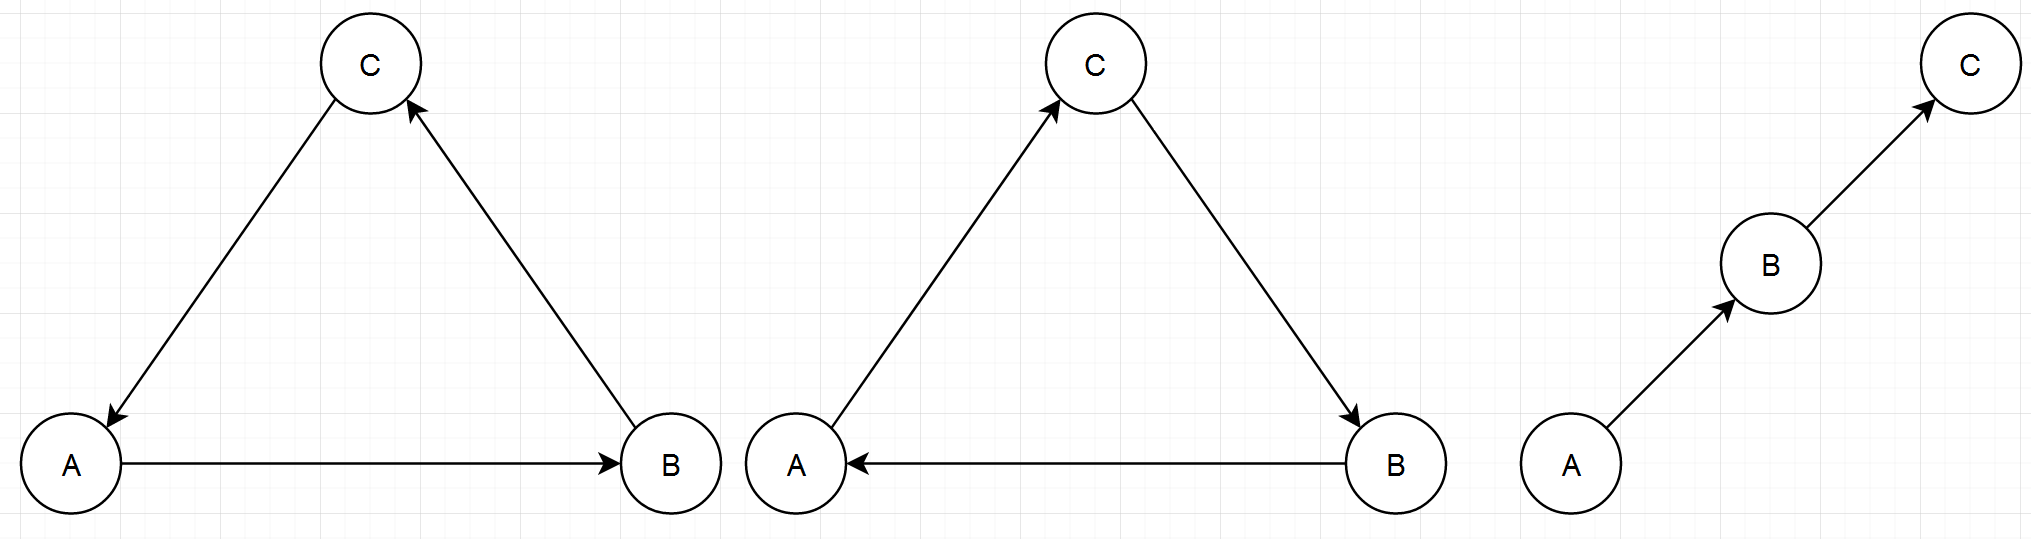
\includegraphics[width=9cm]{Orientation.png}
		\caption{Die drei verschiedenen Orientierungen}
		\label{figure_3}
	\end{center}
\end{figure}
Die Abbildung 1 zeigt die Verschiedenen Orientierungen. Für die Berechnung der Orientierung wird der CCW verwendet:
\[ 
ccw(p,q,r) := 
\begin{vmatrix}
	p_1 & p_2 & 1 \\ 
	q_1 & q_2 & 1 \\ 
	r_1 & r_2 & 1 \notag
\end{vmatrix} \]
\[ ccw = p_1*q_2 - p_2*q_1 + q_1*r_2 - q_2*r_1 + p_2*r_1 - p_1*r_2\]
\[ ccw(p,q,r) \begin{cases} < 0 &\text{r liegt rechts von [p,q]}\\ = 0 &\text{r liegt auf Strahl [p,q]}\\ > 0 &\text{r liegt links von [p,q]}\end{cases} \]
\section{Orientierung der zwei Strecken}
Die zwei Strecken mit den Punkten $(p_1,q_1)$ und $(p_2,q_2)$ schneiden sich wenn der normale Fall oder der Spezialfall bei Kollinearität zutrifft. Sollte keiner der beiden Fälle zutreffen dann schneiden sich beide Strecken nicht.\\
\begin{figure}[h]
	\begin{center}
		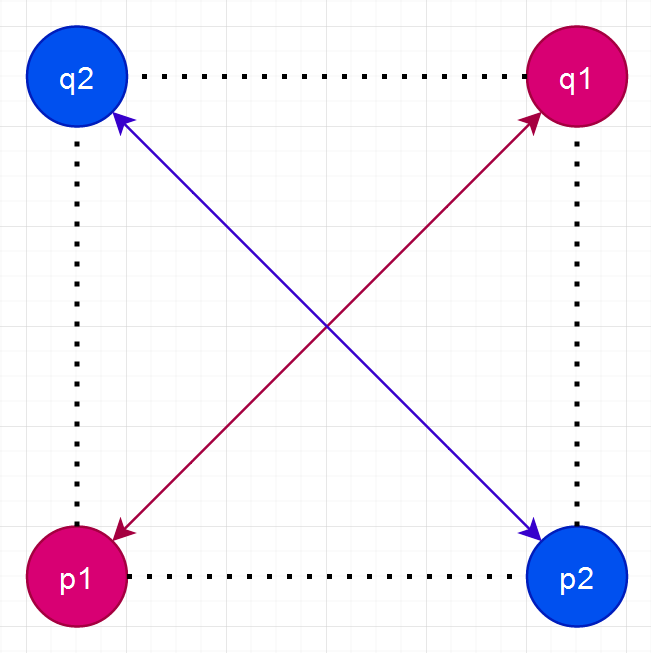
\includegraphics[width=6cm]{Intersection.png}
		\caption{Zwei Strecken die sich schneiden}
		\label{figure_3}
	\end{center}
\end{figure}\\
\subsection{Genereller Fall}
Wenn sich die Orientierungen von $(p_1,q_1,p_2)$ und $(p_1,q_1,q_2)$ unterscheiden und dann die Orientierungen von $(p_2,q_2,p_1)$ und $(p_2,q_2,q_1)$ sich auch unterscheiden, dann müssen sich die beiden Strecken schneiden.\\
\begin{figure}[h]
	\begin{center}
		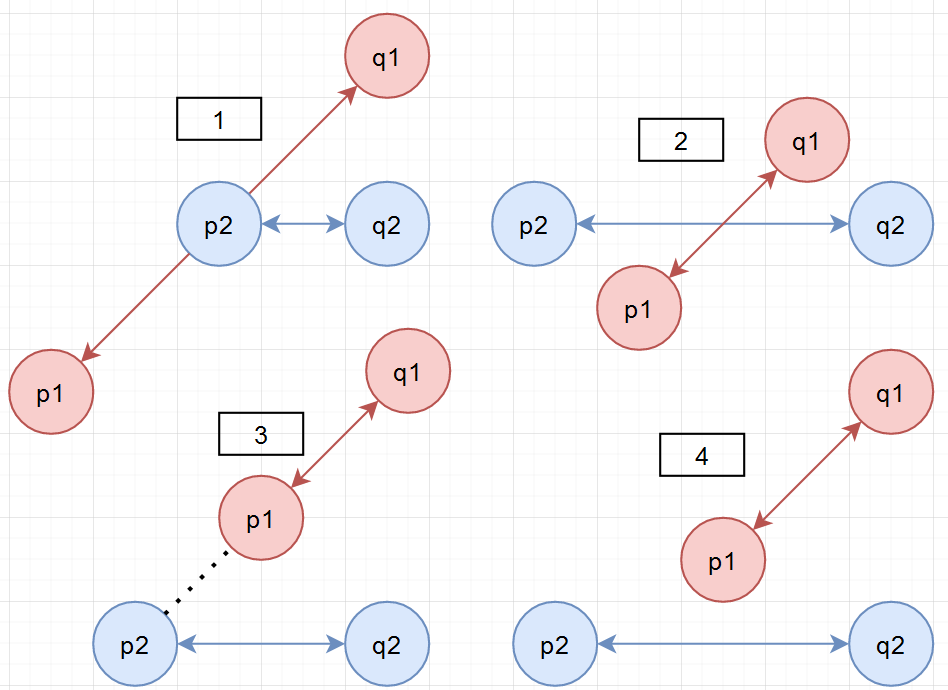
\includegraphics[width=9.3cm]{Cases.png}
		\caption{Alle generellen Fälle}
		\label{figure_3}
	\end{center}
\end{figure}
\begin{enumerate}
	\item Für diesen Fall unterscheiden sich $(p_1,q_1,p_2)$, $(p_1,q_1,q_2)$ und $(p_2,q_2,p_1)$, $(p_2,q_2,q_1)$ $=>$ Sie schneiden sich.
	\item Für diesen Fall unterscheiden sich $(p_1,q_1,p_2)$, $(p_1,q_1,q_2)$ und $(p_2,q_2,p_1)$, $(p_2,q_2,q_1)$ $=>$ Sie schneiden sich.
	\item Für diesen Fall unterscheiden sich $(p_1,q_1,p_2)$, $(p_1,q_1,q_2)$ aber $(p_2,q_2,p_1)$, $(p_2,q_2,q_1)$ sind gleich $=>$ Sie schneiden sich nicht.
	\item Für diesen Fall unterscheiden sich $(p_1,q_1,p_2)$, $(p_1,q_1,q_2)$ aber $(p_2,q_2,p_1)$, $(p_2,q_2,q_1)$ sind gleich $=>$ Sie schneiden sich nicht.
\end{enumerate}
\subsection{Spezial Fall bei Kollinearität}
Wenn $(p_1,q_1,p_2)$, $(p_1,q_1,q_2)$, $(p_2,q_2,p_1)$ und $(p_2,q_2,q_1)$ alle gleich 0 sind, dann sind beide Strecken kollinear. Beide Strecken liegen auf einem Strahl. Jetzt muss noch überprüft werden ob sich die Beiden mindestens in einem Punkt überschneiden.\\
Hierfür werden 4 Prüfungen durchgeführt. Es wurde überprüft ob $p_2$ auf der Strecke $p_1,q_1)$, $q_2$ auf $(p_1,q_1)$, $p_1$ auf $(p_2,q_2)$ und $q_1$ auf $(p_2,q_2)$ liegt. Sollte einer der Punkte auf einer der Strecken liegen gibt es einen Schnittpunkt.
\begin{figure}[h]
	\begin{center}
		\includegraphics[width=6cm]{überlappen.png}
		\caption{Spezialfall bei Kolinearität und Überlappung}
		\label{figure_3}
	\end{center}
\end{figure}
\begin{figure}[h]
	\begin{center}
		\includegraphics[width=6cm]{überlappenNS.png}
		\caption{Spezialfall bei Kolinearität ohne sich zu schneiden}
		\label{figure_3}
	\end{center}
\end{figure}

\subsection{Berechnung ob Strecken sich Überschneiden}
Auch hier werden vier Test durchgeführt. Es wird getestet:
\begin{enumerate}
	\item ob p2 zwischen p1 und q1 liegt,
	\item ob q2 zwischen p1 und q1  liegt,
	\item ob p1 zwischen p2 und q2 liegt,
	\item ob q1 zwischen p2 und q2 liegt.
\end{enumerate}
Sollte einer dieser Fälle zutreffen dann Überlappen sich die beiden Strecken.

 
\section{Ergebnisse}
Die Ergebnisse für die einzelnen Dateien sind:\\
\vspace{0.2cm}\\
\begin{tabular}{|c|c|}
	\hline
	Datei & Schneidende Strecken \\
	\hline
	s\_1000\_1.dat & 11 \\
	\hline
	s\_10000\_1.dat & 732 \\
	\hline
	s\_100000\_1.dat & 77126 \\
	\hline
\end{tabular}
\section{Testen des Algorithmus}
Für die Korrektheit des Program's entwickelte ich 19 Testfälle die weitestgehend alle Fälle abdecken sollten. Es wurde nicht systematisch gegen numerischer Stabilität getestet.\\
\\
Zusätzlich wurde mit einer Vielzahl von Kommilitonen die Zahl der schneidenden Strecken verglichen. Hierbei war die Anzahl identisch. Es ist nicht auszuschließen das alle den selben Fehler gemacht haben.

\section{Ausgleich von Ungenauigkeiten bei Berechnungen mit dem Datentyp Double}
Um Fehler bei Berechnungen mit Double Werten auszugleichen wurde ein kleiner Threshold der Größe $0.0000000001d$ eingebaut. Da in diesem Programm alle Überprüfungen nahe 0 sind ist auch die Genauigkeit der Double Werten sehr hoch. Es wurde auch getestet ob dieser Threshold selbst eine Fehlerquelle ist.

\section{Laufzeitverbesserung des Algorithmus}
Um die Laufzeit des Programm's zu verbessern wurden zwei Wege untersucht.
\subsection{Optimierung der Komplexität des Algorithmus}
Ein naiver Ansatz würde alle Strecken jeweils zweimal vergleichen. So würde mit zwei \textit{for-Schleifen} einmal AB verglichen werden und später nochmal BA. Ein Vergleich einer Strecke mit sich selbst wird nicht durchgeführt da diese sich ohnehin schneiden. Diese Methode würde in einer Komplexität von $\mathcal{O}(n^2-n)$ resultieren.\\
Hier gibt es Verbesserungspotential. So kann man die 2 \textit{for-Schleife} mit dem aktuellen Index der ersten beginnen lassen:
\begin{lstlisting}
int counter = 0;
for(int m = 0 ; m < size ; m++){
	for(int n = m ; n < size; n++){
		if(m!=n){
			if(lines.get(n).isIntersecting(lines.get(m))){
				counter++;
			}
		}
	}
}
\end{lstlisting}
Bei jedem äußeren Schleifendurchgang spart man sich einen weiteren inneren Durchlauf.
Deshalb lässt sich die Komplexität als Summe beschreiben:
\[ \sum_{k=1}^{n} k = 1+2+3+4+5+...+n = (n^2 + n) / 2 \]
Entfernt man dann noch die Vergleiche mit sich selbst kommt man zu $\mathcal{O}(\frac{(n^2 + n)}{2}-n)$\\
Es sollte gelten:
\[ \mathcal{O}(n^2) \geq \mathcal{O}(\frac{(n^2 + n)}{2}-n) \]
Beide liegen aber noch immer in der gleichen Komplexitätsklasse $\mathcal{O}(n^2)$.

\subsection{Parallelisierung}
Um die Laufzeit noch weiter zu verbessern wurde eine Parallelisierung untersucht.\\
Hierbei konnte man ganz einfach den Code parallelisieren indem man Vorteile der Funktionalen Programmierung nutzt. Es werden einfach die gesamte Menge der zu vergleichenden Strecken auf m Kerne verteilt. Die Ergebnisse der einzelnen Threads werden zusammenaddiert. Der Zeitliche Bedarf reduziert sich bei größeren Problemen zunehmend. Bei kleinen Problemen lohnt sich die Parallelisierung wegen des Overheads nicht.\\
\begin{tabular}{|c|c|c|}
	\hline
	Datei & Single & Parallelisiert \\
	\hline
	s\_1000\_1.dat &  &  \\
	\hline
	s\_10000\_1.dat &  &  \\
	\hline
	s\_100000\_1.dat &  &  \\
	\hline
\end{tabular}
\begin{thebibliography}{00}
	\bibitem{b1}http://www.dcs.gla.ac.uk/~pat/52233/slides/Geometry1x1.pdf
\end{thebibliography}

\section{Anhang}

Berechnung ob zwei Strecken sich schneiden:
\begin{lstlisting}
public boolean isIntersecting( Line2Points that){
	final Point start1 = this.start;
	final Point end1 = this.end;
	final Point start2 = that.start;
	final Point end2 = that.end;
	
	final int o1 = orientation(start1, end1, start2);
	final int o2 = orientation(start1, end1, end2);
	final int o3 = orientation(start2, end2, start1);
	final int o4 = orientation(start2, end2, end1);
	
	if (o1 != o2 && o3 != o4)// General Interesction case
	return true;
	
	if (o1 == 0 && o2 == 0 && o3 == 0 && o3 == 0){// If the segments are colinear -> check for overlap
		return onSegment(start1, start2, end1) || onSegment(start1, end2, end1) || onSegment(start2, start1, end2) || onSegment(start2, end1, end2);
	}
	
	return false; // Doesn't fall in any in general or special cases -> No Intersection
}
\end{lstlisting}

Berechnung der Orientierung von drei Punkten:
\begin{lstlisting}
/**
* Find orientation of p, q, r.
* @param p Point
* @param q Point
* @param r Point
* @return 0 -> p, q and r are colinear, 1 -> Clockwise, 2 -> Counterclockwise
*/
private int orientation(Point p, Point q, Point r){
	final double ccw = p.getX()*q.getY() - p.getY()*q.getX() + q.getX()*r.getY() - q.getY()*r.getX() + p.getY()*r.getX() - p.getX()*r.getY();
	
	if(Tool.compareDouble(ccw, 0))
		return 0; // colinear
	else if(ccw > 0)
		return 1; //clockwise
	else
		return 2; //counterclock
}
\end{lstlisting}
	
Berechnung ob ein Punkt auf einer Strecke liegt:
\begin{lstlisting}
// Given three colinear points p, r, q, the function checks if point r lies on line segment 'pq'
private boolean onSegment(Point p, Point r, Point q){
	return r.getX() <= Math.max(p.getX(), q.getX()) &&
	r.getX() >= Math.min(p.getX(), q.getX()) &&
	r.getY() <= Math.max(p.getY(), q.getY()) &&
	r.getY() >= Math.min(p.getY(), q.getY());
}
\end{lstlisting}
	
	
\end{document}
